% Copyright Luke Olson 2009--2014
% This work is licensed under the Creative Commons
% Attribution-NonCommercial-NoDerivatives 4.0 International License. To view a
% copy of this license, visit http://creativecommons.org/licenses/by-nc-nd/4.0/.
%
\documentclass[10pt]{beamer}
%\documentclass[handout,10pt]{beamer}
%pdflatex -jobname lecture15.print lecture15
%
\mode<presentation>
{
  \usetheme[secheader]{Boadilla}
  \usefonttheme[onlymath]{serif}
  \setbeamercovered{invisible}
  \usecolortheme{luke}
  %\setbeamercovered{transparent}
  %
}
\mode<handout>
{
  \usetheme[secheader]{Boadilla}
  \usefonttheme[onlymath]{serif}
  \setbeamercovered{invisible}
  \usecolortheme{luke2}
  %\setbeamercovered{transparent}
}
\usepackage{pgf,pgfarrows,pgfnodes,pgfautomata,pgfheaps,pgfshade}
\usepackage{pxfonts}
\usepackage{eulervm}
\usepackage{listings}
\usepackage{pdfpages}
%\usepackage{pgfpages}
%\pgfpagesuselayout{2 on 1}[letterpaper]
%
%
%%%%%%%%%%%%%%%%%%%%%%%%%%%%%%%%%%%%%%%%%%%%%%%%%%%%%%%%%%%%%%%%%%%%%%%%


%
%
%
\newcommand{\vb}{{\bf{b}}}
\newcommand{\ve}{{\bf{e}}}
\newcommand{\vg}{{\bf{g}}}
\newcommand{\vp}{{\bf{p}}}
\newcommand{\vr}{{\bf{r}}}
\newcommand{\vu}{{\bf{u}}}
\newcommand{\vx}{{\bf{x}}}
\newcommand{\vz}{{\bf{z}}}
\newcommand{\vA}{{\bf{A}}}
\newcommand{\vU}{{\bf{U}}}
\newcommand{\mO}{{\mathcal{O}}}
\newcommand{\mF}{{\mathcal{F}}}
\definecolor{mygray}{rgb}{0.95,0.95,0.95}
\lstset{
        language=matlab,
        numbers=left, numberstyle=\tiny, stepnumber=1, numbersep=5pt,
        basicstyle=\color{black}\ttfamily\small,
        commentstyle=\color{green}\ttfamily,
        keywordstyle=\color{blue}\ttfamily,
        stringstyle=\color{red}\ttfamily,
        showstringspaces=false,
        backgroundcolor=\color{mygray},
        breaklines,
}
\newcommand{\norm}[1]{{\ensuremath{{\|#1\|}}}}
\newcommand{\matdim}[2]{\ensuremath{#1\times#2}}
\newcommand{\rank}[1]{\ensuremath{\mathrm{rank}(#1)}}
\newcommand{\epsm}{\ensuremath{\varepsilon_m}}
\newcommand{\cmd}[1]{{\normalfont\ttfamily\bfseries#1}}

\author{L. Olson}
\institute[UIUC]
{Department of Computer Science\\
University of Illinois at Urbana-Champaign\\
\vspace{0.5cm}
}
%%%%%%%%%%%%%%%%%%%%%%%%%%%%%%%%%%%%%%%%%%%%%%%%%%%%%%%%%%%%%%%%%%%%%%%%
\pgfdeclareimage[height=0.5cm]{university-logo}{./figs/uiuclogo}
\logo{\pgfuseimage{university-logo}}
%%%%%%%%%%%%%%%%%%%%%%%%%%%%%%%%%%%%%%%%%%%%%%%%%%%%%%%%%%%%%%%%%%%%%%%%
\title[CS 357]{Lecture 22}
\subtitle{Google and Markov Chains, Power Method, SVD}
\date{November 12, 2009}

\begin{document}
% -------------------------------------------------
\begin{frame}
  \titlepage
\end{frame}
% -------------------------------------------------
%%%%%%%%%%%%%%%%%%%%%%%%%%%%%%%%%%%%%%%%%%%%%%%%%%%%%%%%%%%%%%%%%%%%%%%%
\begin{frame}
\frametitle{Coming Up}
  \begin{itemize}
    \item Google, Markov Chains, intro to Monte Carlo Simulations
    \item Eigenvalues: SVD, Power Method
    \item Least-Squares
    \item Monte Carlo Simulations
  \end{itemize}
\end{frame}
%%%%%%%%%%%%%%%%%%%%%%%%%%%%%%%%%%%%%%%%%%%%%%%%%%%%%%%%%%%%%%%%%%%%%%%%
\begin{frame}
\frametitle{Google (basics)}
\framesubtitle{many slides courtesy of T. Chartier at Davidson}
\begin{itemize}
  \item A component of Google's success can be
attributed to the PageRank$^{\rm TM}$ algorithm developed by
Google's founders
  \item  algorithm determined entirely by link structure of the WWW
  \item recomputed once a month
  \item involves no content of any Web page
  \item How are the search results ordered?
\end{itemize}
\end{frame}
%%%%%%%%%%%%%%%%%%%%%%%%%%%%%%%%%%%%%%%%%%%%%%%%%%%%%%%%%%%%%%%%%%%%%%%%%
%%%%%%%%%%%%%%%%%%%%%%%%%%%%%%%%%%%%%%%%%%%%%%%%%%%%%%%%%%%%%%%%%%%%%%%%
\begin{frame}
\frametitle{Randomly Walking with Google}

\begin{itemize}
    \item start at any webpage
    \item randomly select a link and follow
    \item repeat
    \item what are the outcomes?
\end{itemize}
\bigskip

The outcomes of such a random walk are:
\begin{itemize}
\item a dead end on a page with no outgoing links
\item a cycle where you end up where you began: known as a \emph{Markov
chain} or \emph{Markov process}.
\item The limiting probability that an infinitely dedicated random
surfer visits any particular page is its PageRank.
\item A page has high rank if other pages with high rank link to
it.
\end{itemize}
\end{frame}
%%%%%%%%%%%%%%%%%%%%%%%%%%%%%%%%%%%%%%%%%%%%%%%%%%%%%%%%%%%%%%%%%%%%%%%%%
%%%%%%%%%%%%%%%%%%%%%%%%%%%%%%%%%%%%%%%%%%%%%%%%%%%%%%%%%%%%%%%%%%%%%%%%
\begin{frame}
\frametitle{Markov Chains}
\begin{itemize}
\item Markov chains can model the behavior of a system that
depends only on the previous experiment or state.
\item That is, the next state of the system depends only on the
current state where the outcome of each experiment is one of a
discrete set of states.
\item Markov chains require a transition matrix, $P$, where
$P(j,i)$ equals the probability of going from state $i$ to state
$j$.
\end{itemize}
\end{frame}
%%%%%%%%%%%%%%%%%%%%%%%%%%%%%%%%%%%%%%%%%%%%%%%%%%%%%%%%%%%%%%%%%%%%%%%%%
%%%%%%%%%%%%%%%%%%%%%%%%%%%%%%%%%%%%%%%%%%%%%%%%%%%%%%%%%%%%%%%%%%%%%%%%
\begin{frame}
\frametitle{Markov chain model of a Broken Machine}

A certain office machine has three states:  Working, Temporarily
Broken, and Permanently Broken.   Each day it is in one of these
states.  The \emph{transition diagram} between the states is shown
below.

\pgfimage[width=1.5in]{./figs/machine}

Therefore, the transition matrix is:
$$P =
\left(%
\begin{array}{lll}
  .9 & .6 & 0 \\
  .095 & .4 & 0 \\
  .005 & 0 & 1 \\
\end{array}%
\right)
$$
\end{frame}
%%%%%%%%%%%%%%%%%%%%%%%%%%%%%%%%%%%%%%%%%%%%%%%%%%%%%%%%%%%%%%%%%%%%%%%%%
%%%%%%%%%%%%%%%%%%%%%%%%%%%%%%%%%%%%%%%%%%%%%%%%%%%%%%%%%%%%%%%%%%%%%%%%
\begin{frame}
\frametitle{Answers via Markov chains}

In our previous model suppose we ask the question:

\begin{block}{}
If the machine is working on Day 1, what is the probability that
it is still functional (that is, not permanently broken) a year
from now?
\end{block}

\end{frame}
%%%%%%%%%%%%%%%%%%%%%%%%%%%%%%%%%%%%%%%%%%%%%%%%%%%%%%%%%%%%%%%%%%%%%%%%%
%%%%%%%%%%%%%%%%%%%%%%%%%%%%%%%%%%%%%%%%%%%%%%%%%%%%%%%%%%%%%%%%%%%%%%%%
\begin{frame}
\frametitle{Stepping through Time with Markov}

We can answer this question by computing the 365'th power of the
transition matrix:

$$P =
\left(%
\begin{array}{lll}
  .9 & .6 & 0 \\
  .095 & .4 & 0 \\
  .005 & 0 & 1 \\
\end{array}%
\right)^{365} =
\left(%
\begin{array}{lll}
    0.1779 & 0.1792 & 0 \\
    0.0284 & 0.0286 & 0 \\
    0.7937 & 0.7922 & 1
\end{array}%
\right)
$$

The first column of this matrix gives the probability of being in
each state on Day 366 (with our assumption that it is working on
Day 1, so $v^{(0)} = [1~0~0]'$).  We see that the probability that
the machine is permanently broken in 0.7937 and so there is about
a 21\% chance that the machine is still functional.
\end{frame}
%%%%%%%%%%%%%%%%%%%%%%%%%%%%%%%%%%%%%%%%%%%%%%%%%%%%%%%%%%%%%%%%%%%%%%%%%
%%%%%%%%%%%%%%%%%%%%%%%%%%%%%%%%%%%%%%%%%%%%%%%%%%%%%%%%%%%%%%%%%%%%%%%%
\begin{frame}
\frametitle{Steady State Solution}

For this Markov chain the steady state solution is the vector
$\textbf{v} = [0~0~1]'$, as we can see by computing the
eigenvalues and eigenvectors.  That is, $P\textbf{v} =
\textbf{v}$.
\bigskip
\bigskip

State 3 (Permanently Broken) is called an {\it absorbing state}.
No matter what state we start in, we will eventually end up in
State 3 with probability 1, and once in State 3 we can never
leave.
\end{frame}
%%%%%%%%%%%%%%%%%%%%%%%%%%%%%%%%%%%%%%%%%%%%%%%%%%%%%%%%%%%%%%%%%%%%%%%%%
%%%%%%%%%%%%%%%%%%%%%%%%%%%%%%%%%%%%%%%%%%%%%%%%%%%%%%%%%%%%%%%%%%%%%%%%
\begin{frame}
\frametitle{Back to Google}
\begin{itemize}
\item Let $W$ be the set of Web pages that can reached by
following a chain of hyperlinks starting from a page at Google.
\item Let $n$ be the number of pages in $W$.
\item The set $W$ actually varies with time, by the end of 2005,
$n$ was over 10 billion.
\item Let $G$ be the $n \times n$ connectivity matrix of $W$, that
is, $G_{i,j}$ is 1 if there is a hyperlink from page $i$ to page
$j$ and 0 otherwise.
\item Let $H$ be $G$ with each row $i$ divided by the number of outgoing links
from node $i$.
\item The matrix $H$ is huge, but very sparse; its number of
nonzeros is the total number of hyperlinks in the pages in $W$.
\end{itemize}
\end{frame}
%%%%%%%%%%%%%%%%%%%%%%%%%%%%%%%%%%%%%%%%%%%%%%%%%%%%%%%%%%%%%%%%%%%%%%%%%
\setbeamertemplate{background canvas}{}
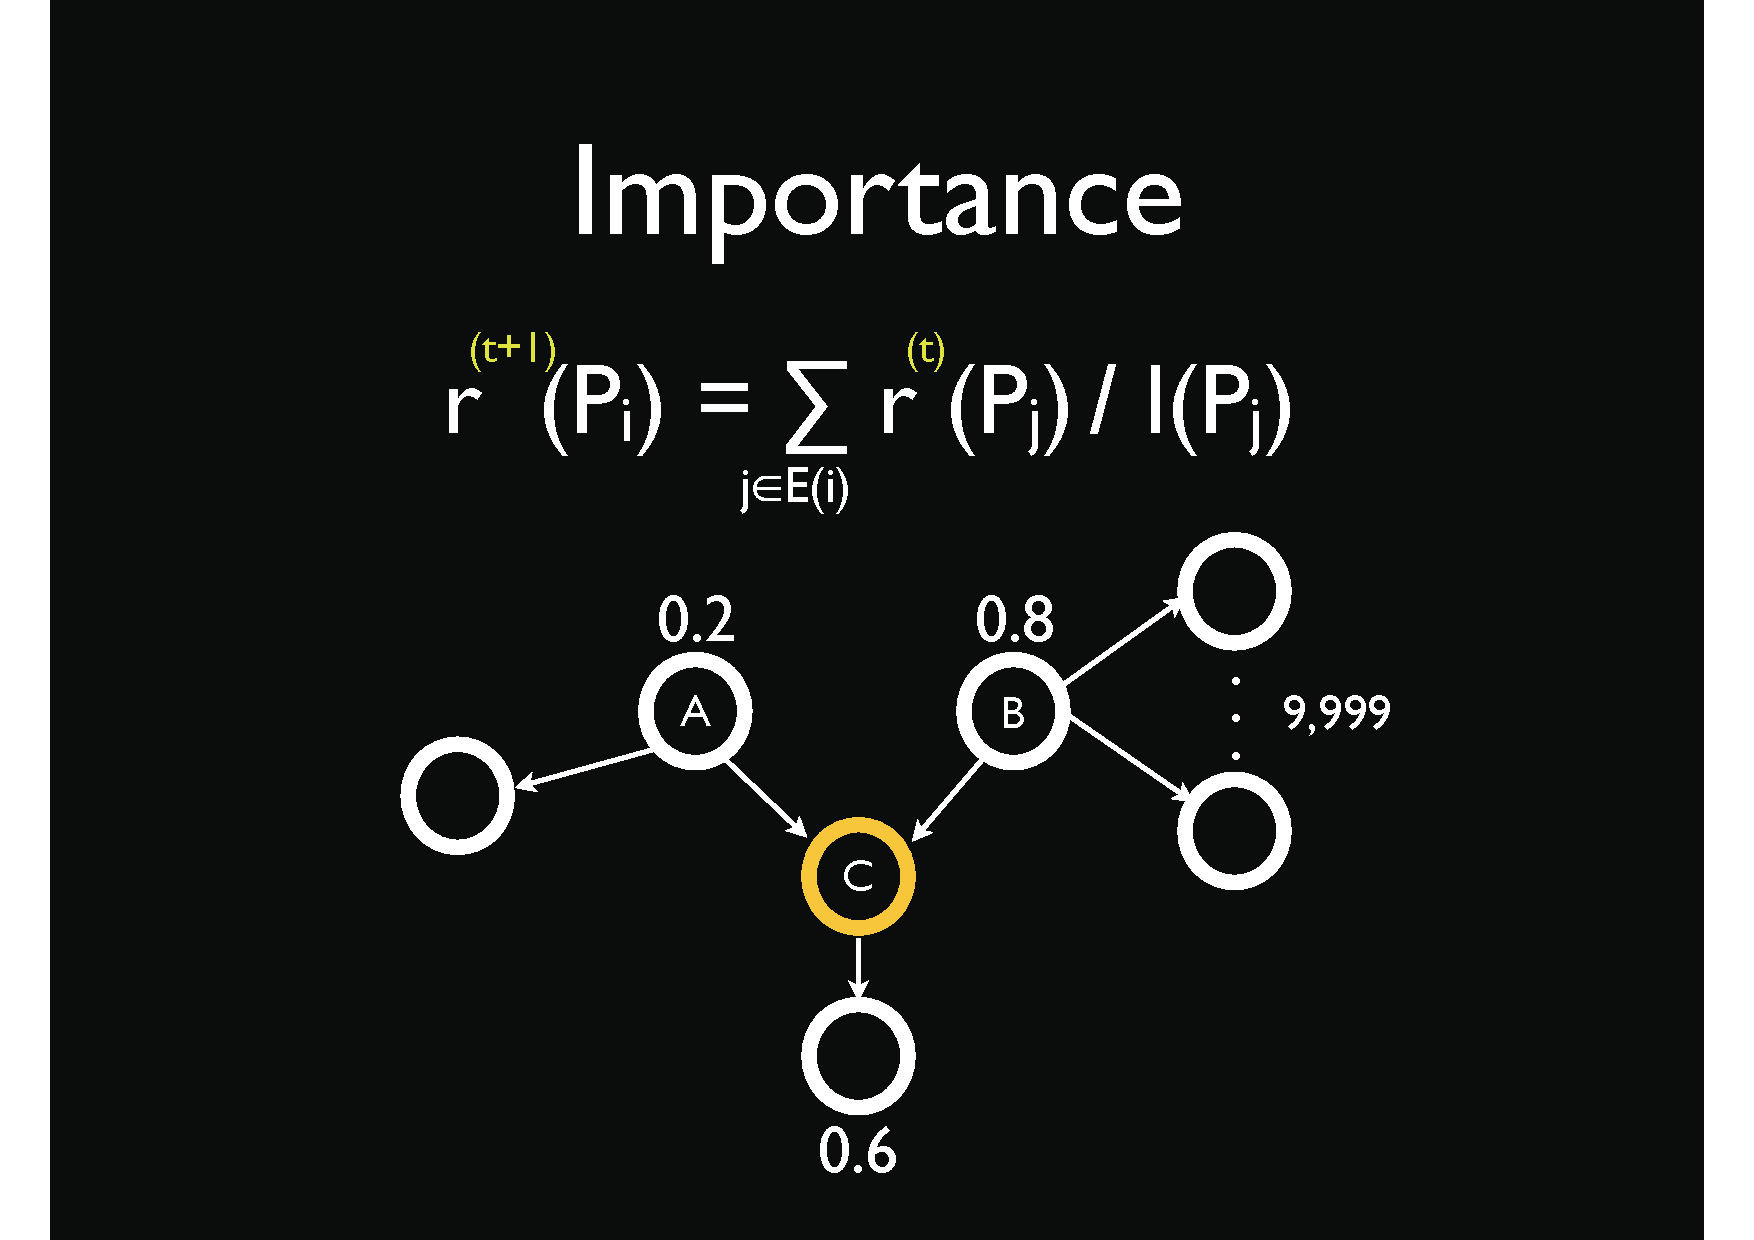
\includepdf[pages=-]{./figs/lecture22_cmu_pagerank.pdf}
%%%%%%%%%%%%%%%%%%%%%%%%%%%%%%%%%%%%%%%%%%%%%%%%%%%%%%%%%%%%%%%%%%%%%%%%
\begin{frame}
\frametitle{Google and Probability}
\begin{itemize}
\item Let $c_j$ and $r_i$ be the column and row sums of $G$,
respectively. That is,
$$c_j = \sum_i G_{i,j}, \qquad r_i = \sum_j G_{i,j}$$
\item Then $c_k$ and $r_k$ are the indegree and outdegree of the
$k$-th page.  In other words, $c_k$ is the number of links into page $k$ 
and $r_k$ is the number of links from page $k$.
\item Let $p$ be the fraction of time that the random walk follows
a link.
\item Google typically takes this to be $p = 0.85$.
\item Then $1-p$ is the fraction of time that an arbitrary page is
chosen.
\end{itemize}
\end{frame}
%%%%%%%%%%%%%%%%%%%%%%%%%%%%%%%%%%%%%%%%%%%%%%%%%%%%%%%%%%%%%%%%%%%%%%%%%
\begin{frame}
\frametitle{Problem}
\begin{itemize}
  \item The power method $x \leftarrow H x$ will converge if $H$ is
\begin{itemize}
\item stochastic: each row is nonnegative with row sum of 1
\item irreducible: possible to get any state from any state
\item aperiodic: every state is periodic with period $k=1$ (self loops)
\end{itemize}
  \item Fix: add these characteristics to the matrix problem
\end{itemize}
\end{frame}
%%%%%%%%%%%%%%%%%%%%%%%%%%%%%%%%%%%%%%%%%%%%%%%%%%%%%%%%%%%%%%%%%%%%%%%%
\begin{frame}
\frametitle{Google meets Markov}
\begin{itemize}
\item Let $A$ be an $n \times n$ matrix whose elements are
$A_{i,j}
= p G_{i,j}/c_j + \delta$ where $\delta = (1-p)/n$.
\item This matrix is the transition matrix of the Markov chain of
a random walk!
\item Notice that $A$ comes from scaling the connectivity matrix
by is column sums.
\item The $j$-th column is the probability of jumping from the
$j$-th page to the other pages on the Web.
\end{itemize}
\end{frame}
%%%%%%%%%%%%%%%%%%%%%%%%%%%%%%%%%%%%%%%%%%%%%%%%%%%%%%%%%%%%%%%%%%%%%%%%%
\begin{frame}
    \frametitle{The problem}
Can write $A$, the transition matrix, as
\[
A = p G D + e z^T
\]
where $e$ is the vector of all ones and where $ez^T$ account for dead linked 
pages and 
\[
D_{jj} = 1/c_j \,\textnormal{(or 0)}\quad z_j = \delta\, \textnormal{(or $1/n$)}
\]
Then $x=Ax$ can be written
\[
 (I-pGD)x = (z^Tx) e = \gamma e
\]
and we can scale $x$ such that $\gamma=1$

see \texttt{pagerank.m}
\end{frame}
%%%%%%%%%%%%%%%%%%%%%%%%%%%%%%%%%%%%%%%%%%%%%%%%%%%%%%%%%%%%%%%%%%%%%%%%
\begin{frame}
\frametitle{Eigenvectors and Google}

Find $x = Ax$ and the elements of $x$ are Google's PageRank.
Remember $n > 10^{10}$ (as of 2005) and growing (a Google blog post
claimed $n > 10^{12}$ in 2008) .
\bigskip
\bigskip

For any particular query, Google finds pages on the Web that match
the query.  The pages are then listed in the order of their
PageRank.
\end{frame}
%%%%%%%%%%%%%%%%%%%%%%%%%%%%%%%%%%%%%%%%%%%%%%%%%%%%%%%%%%%%%%%%%%%%%%%%%
%%%%%%%%%%%%%%%%%%%%%%%%%%%%%%%%%%%%%%%%%%%%%%%%%%%%%%%%%%%%%%%%%%%%%%%%
\begin{frame}
\frametitle{Matlab}
\framesubtitle{Moler's scripts}
To search from a homepage, you will type a statement like:
\bigskip

\texttt{[U,G] = surfer('http://www.uiuc.edu',n)}.
\bigskip

This starts at the given URL and tries to surf the Web until it
has visited $n$ pages.  That is, an $n$ by $n$ matrix is formed.
\bigskip

Note, \texttt{surfer.m} is very primitive...
\end{frame}
%%%%%%%%%%%%%%%%%%%%%%%%%%%%%%%%%%%%%%%%%%%%%%%%%%%%%%%%%%%%%%%%%%%%%%%%%
%%%%%%%%%%%%%%%%%%%%%%%%%%%%%%%%%%%%%%%%%%%%%%%%%%%%%%%%%%%%%%%%%%%%%%%%
\begin{frame}
\frametitle{Matlab}
\framesubtitle{Moler's scripts}
\begin{itemize}
  \item Download \texttt{surfer.m}, \texttt{pagerank.m} and \texttt{pagerankpow.m}

  \item \texttt{[U,G] = surfer('http://www.slashdot.org',20);}
  \begin{description}
    \item[$U$] = a cell array of $n$ strings, the URLs of the nodes.
    \item[$G$]= an $n$-by-$n$ sparse matrix with $G(i,j)=1$ if node $j$
    is linked to node $i$.
  \end{description}
  \item Next: \texttt{spy(G)}.  This shows the nonzero
structure of the connectivity matrix.
  \item Finally: \texttt{pagerank(U,G)} and the pagerank will
be computed.
\end{itemize}
\end{frame}
%%%%%%%%%%%%%%%%%%%%%%%%%%%%%%%%%%%%%%%%%%%%%%%%%%%%%%%%%%%%%%%%%%%%%%%%%
%%%%%%%%%%%%%%%%%%%%%%%%%%%%%%%%%%%%%%%%%%%%%%%%%%%%%%%%%%%%%%%%%%%%%%%%
\begin{frame}
\frametitle{Numerics?}
\begin{itemize}
  \item what does this have to do with numerical methods?
  \item large sparse matrices (although Google avoids this)
  \item solution to a linear system (eigenvalue problem)
  \item Markov chains...
\end{itemize}
The markov process is important.  Let's step back and look at some
statistics
\begin{itemize}
  \item randomness
  \item monte carlo
  \item markov chains
  \item metropolis algorithm
\end{itemize}
Brownian Motion is an example of a Markov process:
\texttt{http://galileo.phys.virginia.edu/classes/109N/more\_stuff/Applets/brownian/brownian.html} (more later)
\end{frame}
%%%%%%%%%%%%%%%%%%%%%%%%%%%%%%%%%%%%%%%%%%%%%%%%%%%%%%%%%%%%%%%%%%%%%%%%%
\begin{frame}
\frametitle{Goal}
  \begin{itemize}
    \item Find $x = Ax$ and the elements of $x$ are Google's PageRank.
    \item For a matrix $A$, the scalar-vector pairs ($\lambda$, $v$) such that
$Av=\lambda v$ are eigenvalue-eigenvectors.
    \item Topic \#1: Power Method
    \item Topic \#2: Singular Value Decomposition (SVD)
  \end{itemize}
\end{frame}
\begin{frame}
\frametitle{Power Method}
Suppose that $A$ is $n \times n$ and that the eigenvalues are ordered:
\[
|\lambda_1| > |\lambda_2| \geq |\lambda_3| \geq \dots \geq |\lambda_n|
\]
Assuming $A$ is nonsingular, we have a linearly independent set of $v_i$ such
that $A v_i = \lambda_i v_i$.
\bigskip

\begin{block}{Goal}
    Computing the value of the largest (in magnitude) eigenvalue, $\lambda_1$.
\end{block}
\end{frame}
\begin{frame}
\frametitle{Power Method}
Take a guess at the associated eigenvector, $x_0$.  We know
\[
x^{(0)} = c_1 v_1 + \dots + c_n v_n
\]
Since the guess was random, start with all $c_j=1$:
\[
x^{(0)} = v_1 + \dots + v_n
\]
Then compute
\begin{align*}
    x^{(1)} & = A x^{(0)}\\
    x^{(2)} & = A x^{(1)}\\
    x^{(3)} & = A x^{(2)}\\
     \vdots & \\
    x^{(k+1)} & = A x^{(k)}\\
\end{align*}
\end{frame}
\begin{frame}
\frametitle{Power Method}
Or $x^{(k)} = A^k x^{(0)}$.  Or
\begin{align*}
    x^{(k)} & = A^k x^{(0)}\\
            & = A^k v_1 + \dots + A^k v_n\\
            & = \lambda_1^k v_1 + \dots \lambda_n^k v_n\\
\end{align*}
And this can be written as
\[
x^{(k)} = \lambda_1^k\left( v_1 + \left(\frac{\lambda_2}{\lambda_1}\right)^k v_2
+ \dots + \left(\frac{\lambda_n}{\lambda_1}\right)^k v_n \right)
\]
So as $k\rightarrow\infty$, we are left with
\[
x^{(k)} \rightarrow \lambda^k v_1
\]
\end{frame}
\begin{frame}[fragile]
\frametitle{The Power Method (with normalization)}
%% We need to explain r and phi in this code - students working from the
%% lecture notes don't have enough info here.
\begin{lstlisting}[mathescape]
for $k=1$ to $kmax$
    $y = Ax$
    $r = \phi(y)/\phi(x)$
    $x = y/\|y\|_{\infty}$
\end{lstlisting}
\begin{itemize}
    \item often $\phi(x) = x_1$ is sufficient
\end{itemize}
\end{frame}
\begin{frame}
\frametitle{Inverse Power Method}
\begin{itemize}
    \item We now want to find the smallest eigenvalue
    \item $Av=\lambda v \quad \Rightarrow \quad A^{-1}v = \frac{1}{\lambda} v$
    \item So ``apply'' power method to $A^{-1}$ (assuming a distinct smallest
eigenvalue)
    \item $x^{(k+1)} = A^{-1} x^{(k)}$
    \item Easier with $A=LU$
    \item Update RHS and backsolve with $U$:
\[
    U x^{(k+1)} = L^{-1} x^{(k)}
\]
\end{itemize}
\end{frame}
%%%%%%%%%%%%%%%%%%%%%%%%%%%%%%%%%%%%%%%%%%%%%%%%%%%%%%%%%%%%%%%%%%%%%%%%
\begin{frame}
\frametitle{SVD: motivation}
% Say something here about problems with Eigenvalues and why we need
% something better.
SVD uses in practice:
\begin{enumerate}
    \item Search Technology: find closely related documents or images in a
database
    \item Clustering: aggregate documents or images into similar groups
    \item Compression: efficient image storage
    \item Principal axis: find the main axis of a solid (engineering/graphics)
    \item Summaries: Given a textual document, ascertain the most representative
tags
    \item Graphs: partition graphs into subgraphs (graphics, analysis)
\end{enumerate}
\end{frame}
\begin{frame}
\frametitle{SVD: Singular Value Decomposition}
SVD takes an $m \times n$ matrix $A$ and factors it:
\[
    A = U S V^T
\]
where $U$ ($m \times m$) and $V$ ($n \times n$) are orthogonal and $S$ ($m
\times n$) is diagonal.

\begin{definition}
    $A$ is orthogonal if $A^TA=AA^T=I$.
\end{definition}

$S$ is made up of ``singular values'':
\[
    \sigma_1 \geq \sigma_2 \geq \dots \geq \sigma_r \geq \sigma_{r+1} = \dots =
\sigma_p = 0
\]
Here, $r=rank(A)$ and $p=min(m,n)$.
\end{frame}
\begin{frame}
\frametitle{Diagonalizing a matrix}
We want to factorize $A$ into $U$, $S$, and $V^T$.  First step: find $V$.
Consider
\[
    A = U S V^T
\]
and multiply by $A^T$
\[
    A^TA = (USV^T)^T (USV^T) = V S^T U^T U S V^T
\]
Since $U$ is orthogonal
\[
    A^T A = V S^2 V^T
\]
This is called a similarity transformation.
\begin{definition}
    Matrices $A$ and $B$ are similar if there is an invertible matrix $Q$ such
that
\[
Q^{-1} A Q = B
\]
\end{definition}
\begin{theorem}
    Similar matrices have the same eigenvalues.
\end{theorem}
\end{frame}
\begin{frame}
\frametitle{Proof}
\begin{align*}
  B v & = \lambda v\\
  Q^{-1} A Q v &= \lambda v\\
  A Q v &= \lambda Q v\\
  A w   &= \lambda w.
\end{align*}
Further, if $v$ is an eigenvector of $B$, $Qv$ is an eigenvector of $A$.
\end{frame}

\begin{frame}
\frametitle{So far...}
Need $A = USV^T$
\bigskip

Look for $V$ such that $A^TA = V S^2V^T$.  Here $S^2$ is diagonal.
\bigskip

If $A^T A$ and $S^2$ are similar, then they have the same eigenvalues.  So the
diagonal matrix $S^2$ is just the eigenvalues of $A^T A$ and $V$ is the matrix
of eigenvectors.
\bigskip
To see the latter, note that since $S^2$ is diagonal, the eigenvectors
are $e_i$, and $V^Te_i$ is just the i$^{th}$ column of $V^T$.

\end{frame}
\begin{frame}
\frametitle{Similarly...}
Now consider
\[
    A = U S V^T
\]
and multiply by $A^T$ from the right
\[
    AA^T = (USV^T) (USV^T)^T = U S V^T V S^T U^T
\]
Since $V$ is orthogonal
\[
    A A^T = U S^2 U^T
\]
Now $U$ is the matrix of eigenvectors of $AA^T$.
\end{frame}
\begin{frame}
\frametitle{In the end...}
We get
\[
A =
\begin{bmatrix}
    \vdots & \vdots & \vdots\\
    u_1    & \dots  & u_m \\
    \vdots & \vdots & \vdots
\end{bmatrix}
\begin{bmatrix}
    \sigma_1 &        &          &        &\\
             & \ddots &          &        & \\
             &        & \sigma_r &        & \\
             &        &          & \ddots & \\
             &        &          &        & 0 
\end{bmatrix}
\begin{bmatrix}
    \dots & v_1^T & \dots\\
    \dots & \vdots & \dots\\
    \dots & v_n^T & \dots
\end{bmatrix}
\]
\end{frame}
\begin{frame}
\frametitle{Example}
Decompose
\[
A = \begin{bmatrix}2 & -2\\ 1 & 1\end{bmatrix}
\]
First construct $A^T A$:
\[
A^TA 
= 
\begin{bmatrix}2 & 1\\ -2 & 1\end{bmatrix}
\begin{bmatrix}2 & -2\\ 1 & 1\end{bmatrix}
=
\begin{bmatrix}
5 & -3\\ -3 & 5
\end{bmatrix}
\]
Eigenvalues: $\lambda_1 = 8$ and $\lambda_2 = 2$.  So
\[
S^2=
\begin{bmatrix}
8 & 0\\ 0 & 2
\end{bmatrix}
\quad
\Rightarrow
\quad
S=
\begin{bmatrix}
2\sqrt{2} & 0\\ 0 & \sqrt{2}
\end{bmatrix}
\]
\end{frame}
\begin{frame}
\frametitle{Example}
Now find $V^T$ and $U$.  The columns of $V^T$ are the eigenvectors of $A^T A$.
\begin{itemize}
    \item $\lambda_1=8$:  $(A^T A - \lambda_1 I) v_1 = 0$
\[
\Rightarrow 
\begin{bmatrix}
-3 & - 3\\
-3 & - 3
\end{bmatrix}
v_1 = 0
\quad
\Rightarrow 
\quad
\begin{bmatrix}
1 & 1\\
0 & 0
\end{bmatrix}
v_1 = 0
\quad
\Rightarrow 
\quad
v_1 = 
\begin{bmatrix}
-1 \\
1
\end{bmatrix}
=
\begin{bmatrix}
-\sqrt{2}/2\\
\sqrt{2}/2
\end{bmatrix}
\]
    \item $\lambda_2=2$:  $(A^T A - \lambda_2 I) v_2 = 0$
\[
\Rightarrow 
\begin{bmatrix}
 3 & - 3\\
-3 &   3
\end{bmatrix}
v_2 = 0
\quad
\Rightarrow 
\quad
\begin{bmatrix}
1 & -1\\
0 & 0
\end{bmatrix}
v_2 = 0
\quad
\Rightarrow 
\quad
v_2 = 
\begin{bmatrix}
1 \\
1
\end{bmatrix}
=
\begin{bmatrix}
\sqrt{2}/2\\
\sqrt{2}/2
\end{bmatrix}
\]
    \item Finally:
\[
V=
\begin{bmatrix}
-\sqrt{2}/2 & \sqrt{2}/2\\
\sqrt{2}/2  & \sqrt{2}/2
\end{bmatrix}
\]
\end{itemize}
\end{frame}
\begin{frame}
\frametitle{Example}
Now find $U$.  The columns of $U$ are the eigenvectors of $A A^T$.
\begin{itemize}
    \item $\lambda_1=8$:  $(A A^T - \lambda_1 I) u_1 = 0$
\[
\Rightarrow 
\begin{bmatrix}
 0 & 0\\
 0 & -6 
\end{bmatrix}
u_1 = 0
\quad
\Rightarrow 
\quad
\begin{bmatrix}
0 & 1\\
0 & 0
\end{bmatrix}
u_1 = 0
\quad
\Rightarrow 
\quad
u_1 = 
\begin{bmatrix}
-1 \\
0
\end{bmatrix}
\]
    \item $\lambda_2=2$:  $(A A^T - \lambda_2 I) u_2 = 0$
\[
\Rightarrow 
\begin{bmatrix}
 6 & 0\\
 0 & 0
\end{bmatrix}
u_2 = 0
\quad
\Rightarrow 
\quad
\begin{bmatrix}
1 & 0\\
0 & 0
\end{bmatrix}
u_2 = 0
\quad
\Rightarrow 
\quad
u_2 = 
\begin{bmatrix}
0 \\
1
\end{bmatrix}
\]
    \item Finally:
\[
U=
\begin{bmatrix}
-1 & 0\\
 0 & 1
\end{bmatrix}
\]

    \item Together:
\[
A = 
\begin{bmatrix}
-1 & 0\\
 0 & 1
\end{bmatrix}
\begin{bmatrix}
2\sqrt{2} & 0\\
        0 & \sqrt{2}
\end{bmatrix}
\begin{bmatrix}
-\sqrt{2}/2 & \sqrt{2}/2\\
 \sqrt{2}/2 & \sqrt{2}/2
\end{bmatrix}
\]
\end{itemize}
\end{frame}
\begin{frame}
\frametitle{SVD: who cares?}
How can we actually \emph{use} $A=USV^T$?  We can use this to represent $A$ with far fewer entries...
\bigskip

Notice what $A=USV^T$ looks like:
\[
    A = \sigma_1 u_1 v_1^T + \sigma_2 u_2 v_2^T + \dots + \sigma_r u_r v_r^T +
0u_{r+1}v_{r+1}^T + \dots + 0u_{p} v_{p}^T
\]
\bigskip

This is easily truncated to
\[
    A = \sigma_1 u_1 v_1^T + \sigma_2 u_2 v_2^T + \dots + \sigma_r u_r v_r^T
\]
\bigskip

see \texttt{svd\_test.m}

What are the savings?  
\begin{itemize}
    \item $A$ takes $m\times n$ storage
    \item using $k$ terms of $U$ and $V$ takes $k(1 + m + n)$ storage
\end{itemize}
\end{frame}
\end{document}
